\subsection{LETs based on organic thin films}\label{sec:thinfilms} %Armin|Cees
Some of the most advantageous properties of organic materials used for photoelectronic devices are easy and cheap fabrication. They can for instance be deposited on many different type of surfaces such as a CMOS or cheap materials like plastic and glass. This can result in lower cost devices, especially because organic materials can be produced with low-cost, large scale industrial production processes such as direct printing, ink-jet and other solution based ones. These features make organic thin film devices best suitable for markets were low-cost production is of high importance and the requirements for high performance do not require inorganic devices. (moet/kan nog een stukje tussen over bron 22-25)

OLEDs are very well known and widely used in low-voltage-driven light-emitting devices, possibly produced on flexible substrates. Where OLETs could produce electroluminescence with the same materials al OLEDs the driving scheme behind it is very different. The main difference is that charge transport in OLEDs occurs perpendicular and through the plane of different layers. Whereas in OLETs charge transport occurs parallel and through the plane. An schematic representation is shown in figure \ref{fig:thinfilms}.

\begin{figure}[!ht]
 \begin{center}
  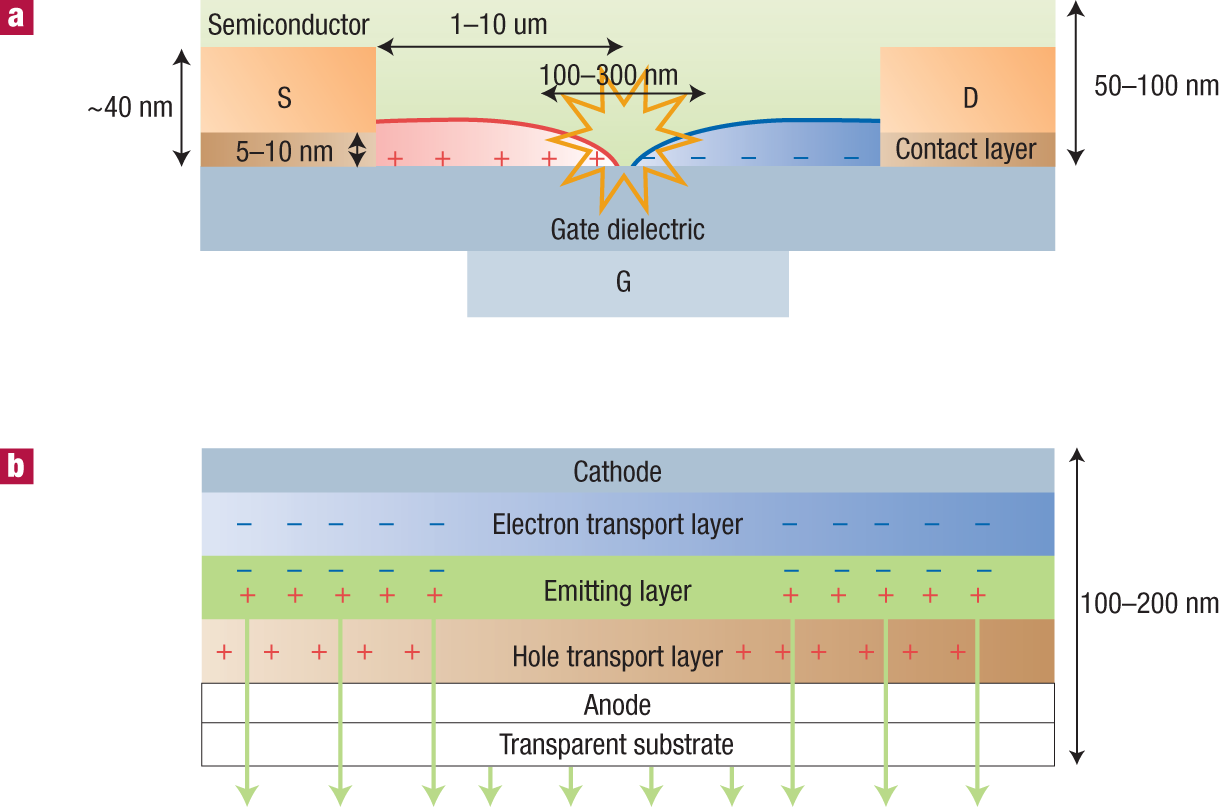
\includegraphics[width=0.8\textwidth]{fig_2}
  \caption{Schematic representation of OLET and OLED. (a) Horizontal charge transport in OLETs. (b) Vertical charge transport in OLEDs. Picture from \citet{Muccini}.}
  \label{fig:thinfilms}
 \end{center}
\end{figure}

For the OLEDs the charge transport is bulk charge transport, for the OLETs it is field-effect charge transport [26]. An other large difference is the distance the minority carriers are required to travel before encountering a charge of the opposite sign and recombine radiatively. In OLEDs the distance the charges have to travel are in the order of few tens of nanometers where for a typical ambipolar OLET the distance is in the order of hundreds nanometers or a few micrometers. This larger distance requires stricter charge transport properties of materials. (iets met electroluminces quantum efficiency).

Due to the device structure (the spacial distance between the exciton formation region and the metal electrodes is much larger in OLETs), OLETs are less affected by electron-metal quenching by interaction with charge carriers. This effect is further reduced by the availability of a third electrode that balances electron and hole currents. These structural advantages make OLETs more favourable for high-brightness electroluminescence and highly integrated devices. These advantages however do rely on development of organic materials.
